\documentclass[a4paper, 12pt]{report}
\usepackage[T1]{fontenc}
\usepackage[utf8]{inputenc}
\usepackage[english]{babel}
\usepackage{mathtools}
\usepackage{amsfonts}
\usepackage{amsmath}
\usepackage{mathrsfs}
\usepackage{enumitem}
\usepackage{booktabs}
\usepackage{array}
% Avoid paragraph indent
\setlength{\parindent}{0pt}
% Useful floor and ceiling functions
\DeclarePairedDelimiter{\floor}{\lfloor}{\rfloor}
\DeclarePairedDelimiter{\ceil}{\lceil}{\rceil}
% Argmax/Argmin notation
\DeclareMathOperator*{\argmax}{argmax} 
\DeclareMathOperator*{\argmin}{argmin} 
% Modified margins
\usepackage[margin=2cm]{geometry}
% This avoids hypenation
\hyphenpenalty=10000
\usepackage{tikz}
\usetikzlibrary{arrows,calc,positioning,shadows,shapes}
\usepackage{graphicx}
\usepackage{subfig}
\captionsetup[figure]{labelfont={bf},name={Figure},labelsep=period}
\captionsetup[table]{labelfont={bf},name={Table},labelsep=period}

\usepackage{float}

\begin{document}
	
\title{Digital Communications and Laboratory \\ Third Homework}
\author{Faccin Dario, Santi Giovanni}
\date{}
\maketitle


\section*{PROBLEM}
The following system was considered. A stream of QPSK symbols is upsampled with period T/4 and filtered with a filter $q_c$ which output is $s_c\left(n\frac{T}{4}\right)= \alpha s_c\left((n-1)\frac{T}{4}\right)+\beta a_{n-5}'$. This signal is transmitted through the channel, which introduces the noise component $w_c\left(n\frac{T}{4}\right)$ with PSD $\mathcal{P}_{w_c}(f) = N_0$. Note that noise components are iid with \textit{pmd} $\sim \mathcal{CN}(0,\sigma_{w_c}^2)$. The SNR at the output of the system is therefore 
\begin{equation*}
\Gamma = \frac{M_{s_c}}{N_0\frac{1}{T}} = \frac{\sigma^2_a E_{q_c}}{\sigma_{w_c}^2}
\end{equation*}
with $\sigma^2_a=2$ and $E_{q_c} = \sum_m | q_c \left(m\frac{T}{4}\right) |^2$.

\begin{figure}[H]
	\centering
	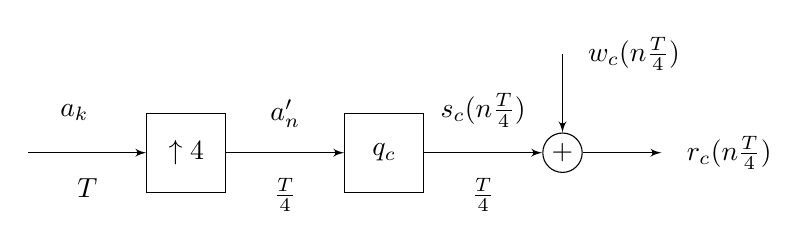
\begin{tikzpicture}[auto,>=latex']
	\tikzstyle{block} = [draw, rectangle, minimum height=1cm, minimum width=1cm]
	
	\node [coordinate, label={[label distance=0.4cm]45:$a_k$}] (start) {};
	\node [block, right = 1.5cm of start] (intpl){$\uparrow 4$};
	\node [coordinate, label={[label distance=0.2cm]90:$a'_n$}, right = 0.75 cm of intpl] (c1) {};
	\node [block, right = 1.5cm of intpl] (imp){$q_c$};
	\node [draw, circle,minimum size=0.5cm,inner sep=0pt, right = 1.5cm of imp] (sum){$+$};
	\node [coordinate, label={[label distance=0.2cm]90:$s_c(n \frac{T}{4})$}, right = 0.75cm of imp] (c2) {};
	
	\node [coordinate, label={[label distance=0.2cm]0:$w_c(n \frac{T}{4})$}, above = 1cm of sum] (wgn) {};
	\node [coordinate, label={[label distance=0.2cm]0:$r_c(n \frac{T}{4})$}, right = 1cm of sum] (end) {};
	
	\draw [->] (start) --node[label={[label distance=0.2cm]270:$T$}]{} (intpl);
	\draw [->] (intpl) --node[label={[label distance=0.2cm]270:$\frac{T}{4}$}]{} (imp);
	\draw [->] (imp) --node[label={[label distance=0.2cm]270:$\frac{T}{4}$}]{} (sum);
	\draw [->] (wgn) --node[]{} (sum);
	\draw [->] (sum) --node[]{} (end);
	
	\end{tikzpicture}
	\caption{Model for the transmission system of Problem 1.}
	\label{Model_1} 
\end{figure}

The QPSK symbols are generated with a PN sequence of length $L=2^{20}-1$ in order to provide a stream of bits with spectral characteristics similar to those of a white noise signal. Two consecutive bits are then coupled and mapped into one of the possible constellations symbols, associating the first and second bit to the real and imaginary part respectively. \\
The $q_c$ filter in linear and frequency domain is given in Figure [\ref{qc}].

\begin{figure}[H]
	\centering
	\subfloat{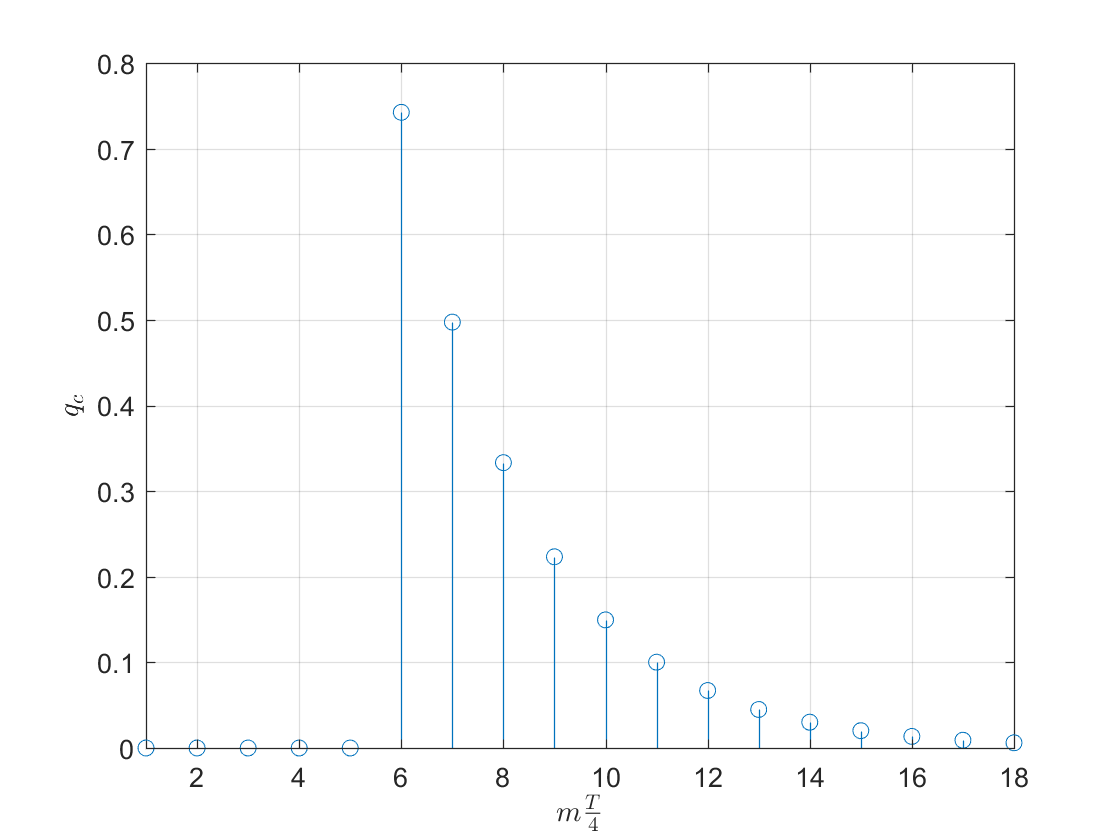
\includegraphics[width=9cm]{images/qc}}
	\subfloat{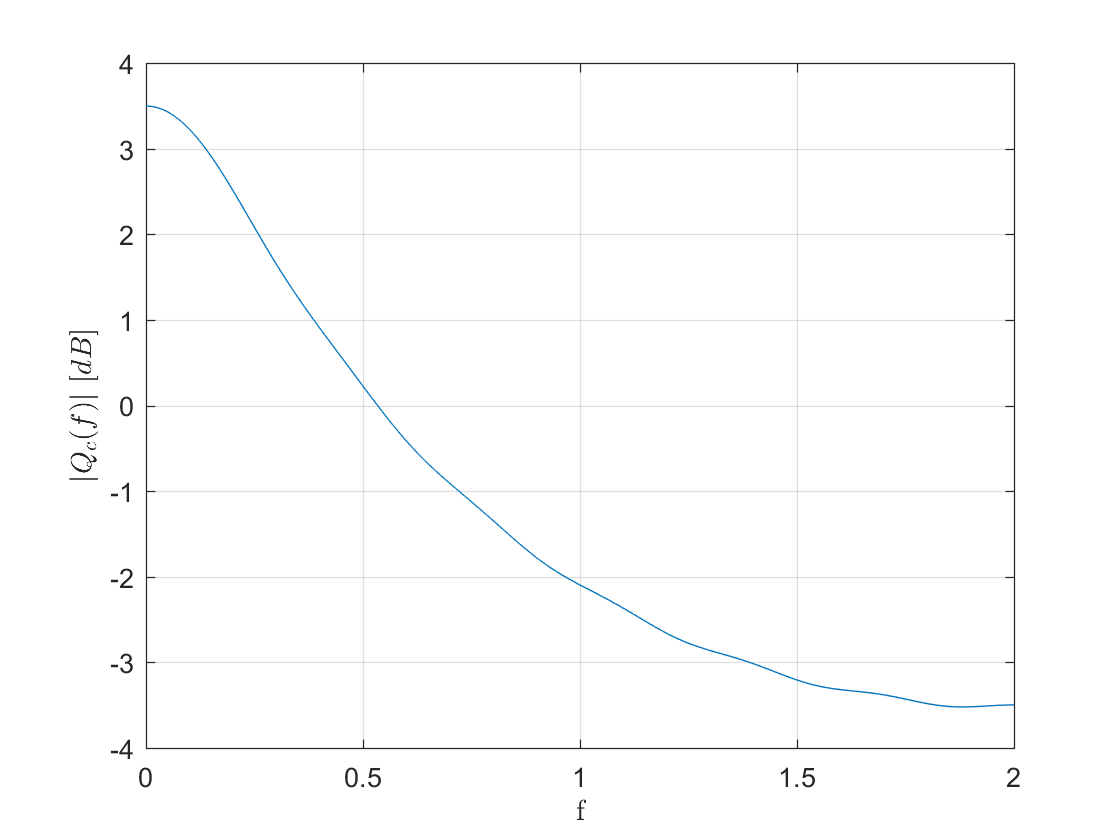
\includegraphics[width=9cm]{images/Qc_f}}
	\caption{Impulse response (left) and Frequency response (right) of the filter $q_c$.}\label{qc}
\end{figure}

In the following, 6 different receiver configurations are analyzed. For each of this, SNR value of $\Gamma = 10$ $dB$ is assumed.

\clearpage

\subsection*{Channel equalization}
Receivers (a), (b), (c) and (d) implement a technique called \textit{Decision feedback equalizer} (DFE) which attempts to reduce the intersymbol interference (ISI).\\
The desired signal at the receiver input is
\begin{equation*}
x_k = \sum_{i=-\infty}^{\infty} a_i h_{k-i} + \tilde{w}_k
\end{equation*}
where $h_n = h_{Tx}*g_C * g_M(t)$. Assuming $\{h_n\}$ has finite duration and support $[-N_1, -N_1+1, \dots, N_2-\, N_2]$, we define \textit{postcursors} the samples with positive index and \textit{precursors} those with negative index.\\
Writing $x_k$ explicitly we can see that it depends both on previous and future symbols.\\
The DFE is composed by two filters:
\begin{enumerate}
	\item \textit{Feedforward (FF) filter c}, with $M_1$ coefficients:
	\begin{equation}
	x_{FF,k} = \sum_{i=0}^{M_1-1}c_ix_{k-i}
	\end{equation}\label{eq:ff_filter}
	\item \textit{Feedback (FB) filter b}, with $M_2$ coefficients:
	\begin{equation}
	x_{FB,k} = \sum_{i=1}^{M_2}b_i a_{k-i-D}
	\end{equation}\label{eq:fb_filter}
\end{enumerate}

Ideally the task of the FF filter is to obtain an overall impulse response $\{\psi_n = h * c_n\}$ with small precursors, while the FB filter should cancel almost all the remaining ISI.\\
The output of the DFE can be written as
\begin{equation}
	\begin{split}
	y_k &= x_{FF,k} + x_{FB,k} \\
	&= \sum_{i=0}^{M_1-1}c_ix_{k-i} + \sum_{j=1}^{M_2}b_ja_{k-D-j}
	\end{split} 
\end{equation}

The Wiener filter theory can be exploited to determine the optimum coefficients, which minimize the cost function
\begin{equation}
J = E \left[|a_{k-D}-y_k|^2\right]
\end{equation}
The optimum FF filter $c$ is given by
\begin{equation}\label{c}
\mathbf{c}_{opt} = \mathbf{R}^{-1}\mathbf{p}
\end{equation}
where the matrices $\mathbf{R}$ and $\mathbf{p}$ are computed using
\begin{equation}
\mathbf{[R]}_{p,q} = \sigma_a^2 \left( \sum_{j=-N_1}^{N_2}h_jh^*_{j-(p-q)}-\sum_{j=1}^{M_2}h_{j+D-q}h^*_{j+d-p} \right) + r_{\tilde{w}}(p-q)
\end{equation}
\begin{equation}
\mathbf{[p]}_p = \sigma_a^2 h^*_{D-p}, \hspace*{4cm} p,q = 0,1,\dots,M_1-1
\end{equation}

The optimum FB coefficients $\{b_i\}$ are given by
\begin{equation}
b_i = -\sum_{l=0}^{M_1-1}c_{opt,l}h_{i+D-l} \hspace*{4cm} i =1,2,\dots,M_2
\end{equation}

The minimum-cost function can be expressed in close form as:
\begin{equation}\label{jmincf}
J_{min} = \sigma^2_a \left( 1-\sum_{l=0}^{M_1-1} c_{opt,l}h_{D-l}\right)
\end{equation}

\subsection*{Receiver a}
\begin{figure}[H]
	\centering
	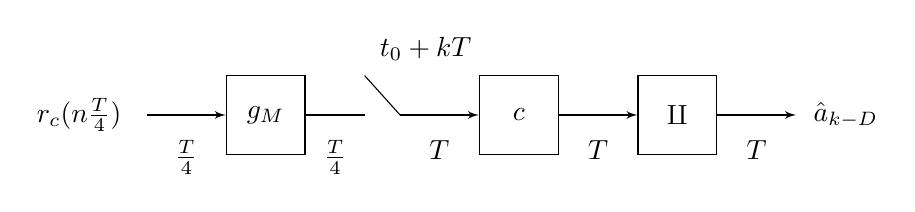
\begin{tikzpicture}[auto,>=latex']
	\tikzstyle{block} = [draw, rectangle, minimum height=1cm, minimum width=1cm]
	
	\node [coordinate, label={[label distance=0.2cm]180:$r_c(n \frac{T}{4})$}] (start) {};
	\node [block, right = 1cm of start] (matchedf){$g_M$};
	\node [coordinate, right = 0.75 cm of matchedf] (c0) {};
	\node [coordinate, above = 0.5 cm of c0, label={[label distance=0.1cm]45:$t_0 + kT$} ] (c1) {};
	
	\node [coordinate, right = 1.2cm of matchedf] (c2) {};
	
	\node [block, right = 1cm of c2] (cfilter){$c$};
	\node [block, right = 1cm of cfilter] (detector){$\amalg$};
	
	\node [coordinate, right = 1cm of detector, label={[label distance=0.1cm]0:$\hat{a}_{k-D}$}] (end){};
	
	\draw [->] (start) --node[label={[label distance=0.2cm]270:$\frac{T}{4}$}]{} (matchedf);
	\draw [-] (matchedf) --node[label={[label distance=0.2cm]270:$\frac{T}{4}$}]{} (c0);
	\draw [-] (c1) --node[]{} (c2);
	\draw [->] (c2) --node[label={[label distance=0.2cm]270:$T$}]{} (cfilter);
	\draw [->] (cfilter) --node[label={[label distance=0.2cm]270:$T$}]{} (detector);
	\draw [->] (detector) --node[label={[label distance=0.2cm]270:$T$}]{} (end);
	
	\end{tikzpicture}
	\caption{Model for the receiver (a).}
	\label{Receiver_a} 
\end{figure}

The receiver filter consists of a filter $g_M$ matched to the transmission filter $q_c$ followed by a \textit{Linear Equalizer (LE) filter} $c$. The matched filter is simply computed as $g_m(t) = q^*_c(t_0-t)$, where $t_0$ is the timing phase. It is given in Figure [\ref{gm_a}]. From now on, we may refer to the global impulse response of the system at the input of  $c$ as $h = g_c * g_M$. Since it is defined @$\frac{T}{4}$, a downsampling of a factor 4 is required between the output of $h$ and the input of $c$. \\
The filter $c$ corresponds to the Feedforward (FF) filter $c$ of Equation (\ref{eq:ff_filter}). Since the LE can be seen as a particular case of a DFE where $M_2 =0$, we developed the general DFE algorithm and set $\{b_i\}=0$ in this case. \\
The equalizer filter $c$ and the overall impulse response $\psi_i=h*c_i$ for SNR of $\Gamma = 10$ dB are given in Figure [\ref{filters_a}]. 

To choose suitable $M_1$, $M_2$ and $D$ we decided to evaluate the functional $J_{min}$ according to Equation (\ref{jmincf}).\\
In Figure [\ref{j_min_le}] we can see that for values greater than $M_1=6$ and $D=4$ there is no noticeable improvement in the cost function, so we decided to use these parameters.

\begin{figure}[H]
	\centering
	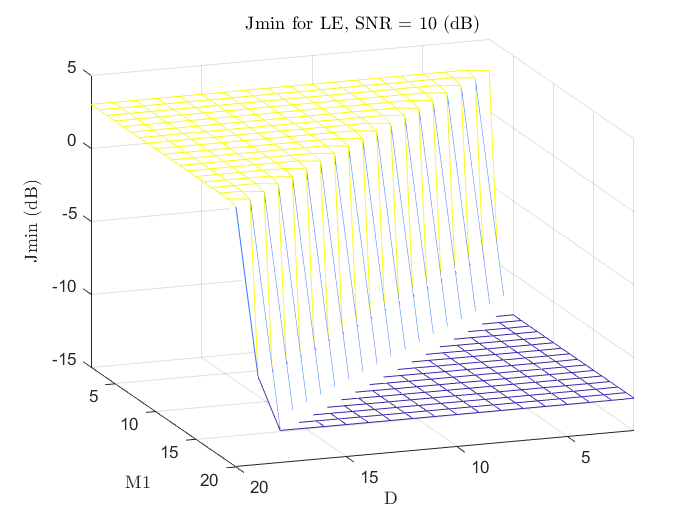
\includegraphics[width=8cm]{images/optimal_params_LE}
	\caption{$J_{min}$ as a function of $M_1$ and $D$.}\label{j_min_le}
\end{figure}

The parameters we obtained are reported in Table [\ref{Tab_a}].

\begin{table}[H]
	\centering
	\begin{tabular}{c c c c}
		\toprule
		$\mathbf{\bar{t}_0}$ & $\mathbf{M_1}$ & $\mathbf{M_2}$ & \textbf{D}     \\
		\midrule
		17 & 6 & 0 & 4 \\
		\bottomrule			
	\end{tabular}
	\caption{Parameters of the Receiver (a).}
	\label{Tab_a}
\end{table}

\begin{figure}[H]
	\centering
	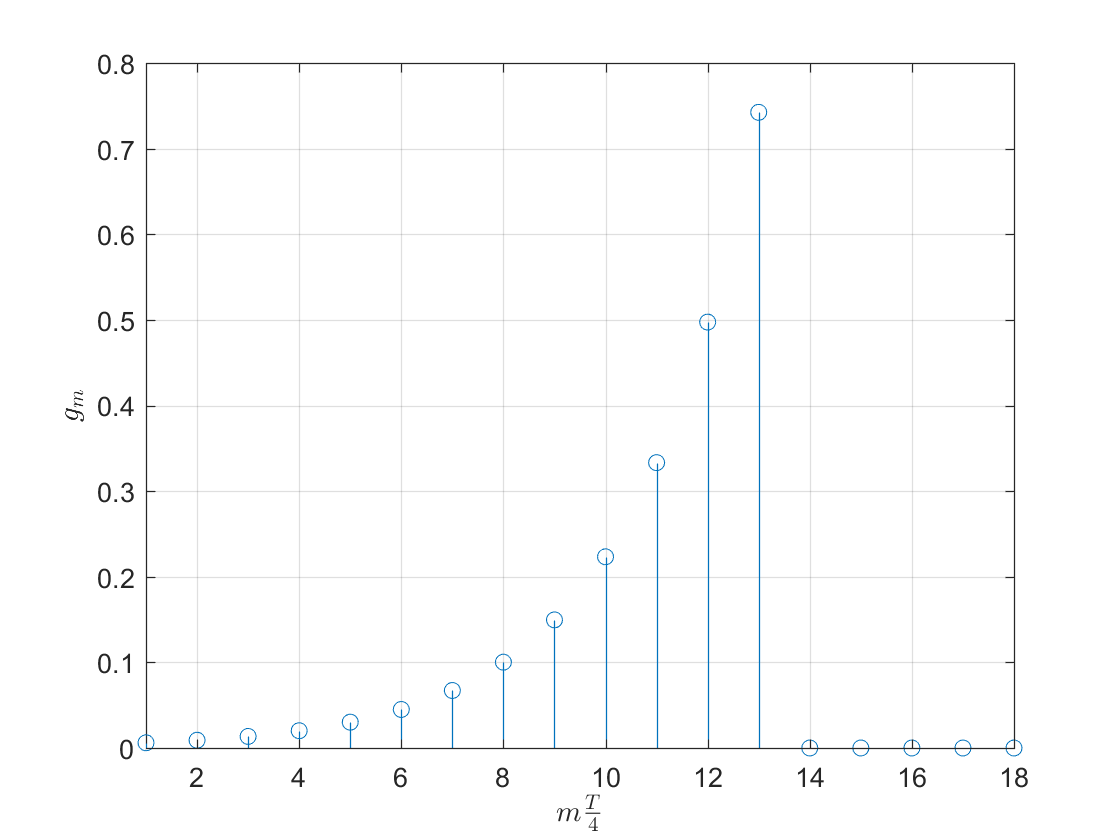
\includegraphics[width=8cm]{images/RecA_gm}
	\caption{Matched filter $g_m$ of the receiver filter.}\label{gm_a}
\end{figure}

\begin{figure}[H]
	\centering
	\subfloat[Equalizer filter $c$]{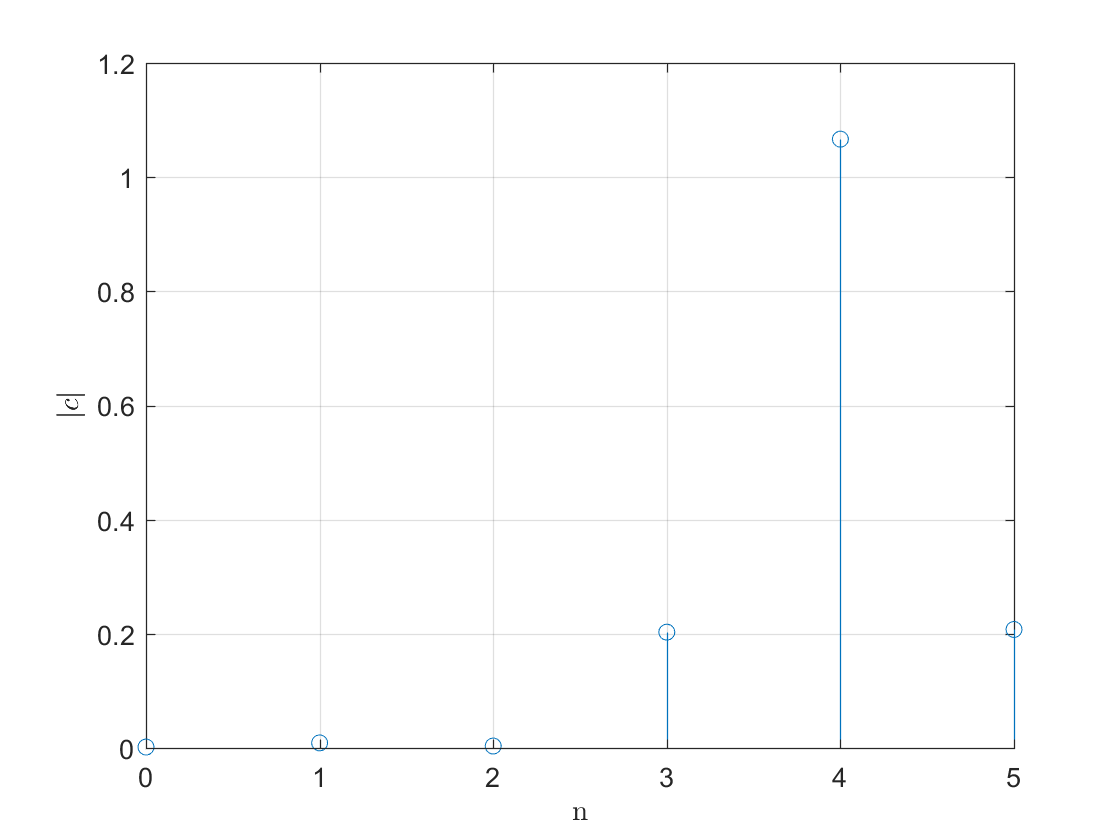
\includegraphics[width=8cm]{images/RecA_c}}
	\subfloat[Overall impulse response $\psi_i$]{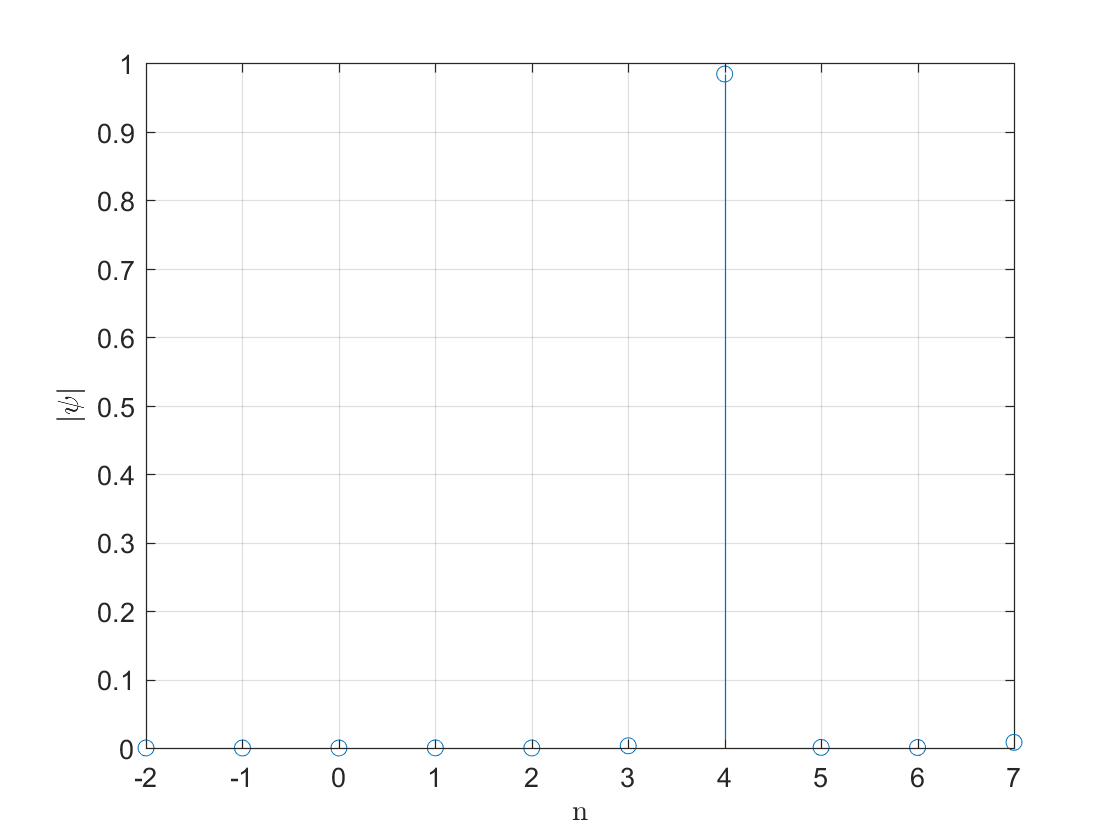
\includegraphics[width=8cm]{images/RecA_psi}}
	\caption{Coefficients of the equalizer filter $c$ and of the overall impulse response $\psi_i$.}\label{filters_a}
\end{figure}

The final signal at the output of the equalizer filter is processed by a threshold detector, which maps each received symbol according to the following rule:

\begin{equation*}
\tilde{a}_k \mapsto \hat{a}_k = \text{sgn}(\Re[\tilde{a}_k ]) +i \cdot \text{sgn}(\Im[\tilde{a}_k ])
\end{equation*}
 
Note that the actual transmitted symbol at time $k$ is detected at time $k+D$ because of the delay introduced by the filter $c$. This detection configuration will be used also for receivers $b$, $c$ and $d$. 

\clearpage

\subsection*{Receiver b}

\begin{figure}[H]
	\centering
	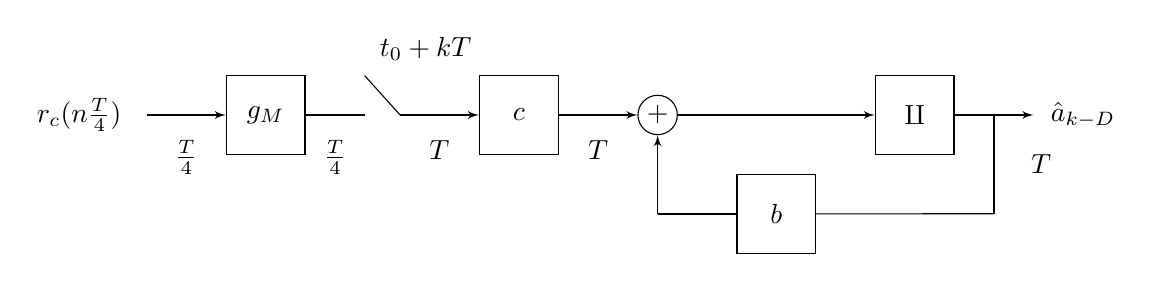
\begin{tikzpicture}[auto,>=latex']
	\tikzstyle{block} = [draw, rectangle, minimum height=1cm, minimum width=1cm]
	
	\node [coordinate, label={[label distance=0.2cm]180:$r_c(n \frac{T}{4})$}] (start) {};
	\node [block, right = 1cm of start] (matchedf){$g_M$};
	\node [coordinate, right = 0.75 cm of matchedf] (c0) {};
	\node [coordinate, above = 0.5 cm of c0, label={[label distance=0.1cm]45:$t_0 + kT$} ] (c1) {};
	
	\node [coordinate, right = 1.2cm of matchedf] (c2) {};
	
	\node [block, right = 1cm of c2] (cfilter){$c$};
	
	\node [draw, circle,minimum size=0.5cm,inner sep=0pt, right = 1cm of cfilter] (sum){$+$};
	
	\node [coordinate, below = 1cm of sum] (c3) {};	
	
	\node [block, right = 2.5cm of sum] (detector){$\amalg$};
	
	\node [coordinate, right = 0.5cm of detector] (cfin) {};
	
	\node [coordinate, below = 1.254cm of cfin] (c6) {};
	
	\node [block, right = 1cm of c3] (b){$b$};	
	
	\node [coordinate, right = 1cm of detector, label={[label distance=0.1cm]0:$\hat{a}_{k-D}$}] (end){};
	
	\draw [->] (start) --node[label={[label distance=0.2cm]270:$\frac{T}{4}$}]{} (matchedf);
	\draw [-] (matchedf) --node[label={[label distance=0.2cm]270:$\frac{T}{4}$}]{} (c0);
	\draw [-] (c1) --node[]{} (c2);
	\draw [->] (c2) --node[label={[label distance=0.2cm]270:$T$}]{} (cfilter);
	\draw [->] (cfilter) --node[label={[label distance=0.2cm]270:$T$}]{} (sum);
	\draw [->] (c3) --node[]{} (sum);
	\draw [-] (b) --node[]{} (c3);
	\draw [-] (c6) --node[]{} (b);
	\draw [-] (cfin) --node[label={[label distance=0.1cm]0:$T$}]{} (c6);
	\draw [->] (sum) --node[]{} (detector);
	\draw [->] (detector) --node[]{} (end);
	\end{tikzpicture}
	\caption{Model for the receiver (b).}
	\label{Receiver_b} 
\end{figure}

The only difference with respect to Receiver (a) is that now the DFE has both the FF filter $c$ of Equation (\ref{eq:ff_filter}) and the FB filter $b$ of Equation (\ref{eq:fb_filter}).\\
As before, to choose the parameters $M_1$, $M_2$ and $D$ we evaluated $J_{min}$ according to Equation (\ref{jmincf}).\\
As in previous configuration we can see that for values greater than $M_1=6$ and $D=4$ there is no noticeable improvement in the cost function, so we decided to use these parameters.

\begin{figure}[H]
	\centering
	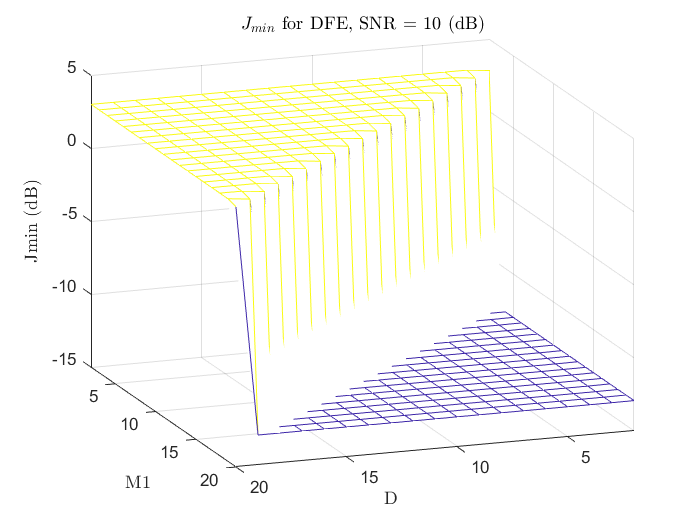
\includegraphics[width=8cm]{images/optimal_params_DFE}
	\caption{$J_{min}$ as a function of $M_1$ and $D$.}\label{j_min_dfe}
\end{figure}

\begin{table}[H]
	\centering
	\begin{tabular}{c c c c}
		\toprule
		$\mathbf{\bar{t}_0}$ & $\mathbf{M_1}$ & $\mathbf{M_2}$ & \textbf{D}     \\
		\midrule
		17 & 6 & 3 & 4 \\
		\bottomrule			
	\end{tabular}
	\caption{Parameters of the Receiver (b).}
	\label{Tab_b}
\end{table}

Using the same algorithm as previous case, we obtained the following filters.

\begin{figure}[H]
	\centering
	\subfloat[Feedforward filter $c$.]{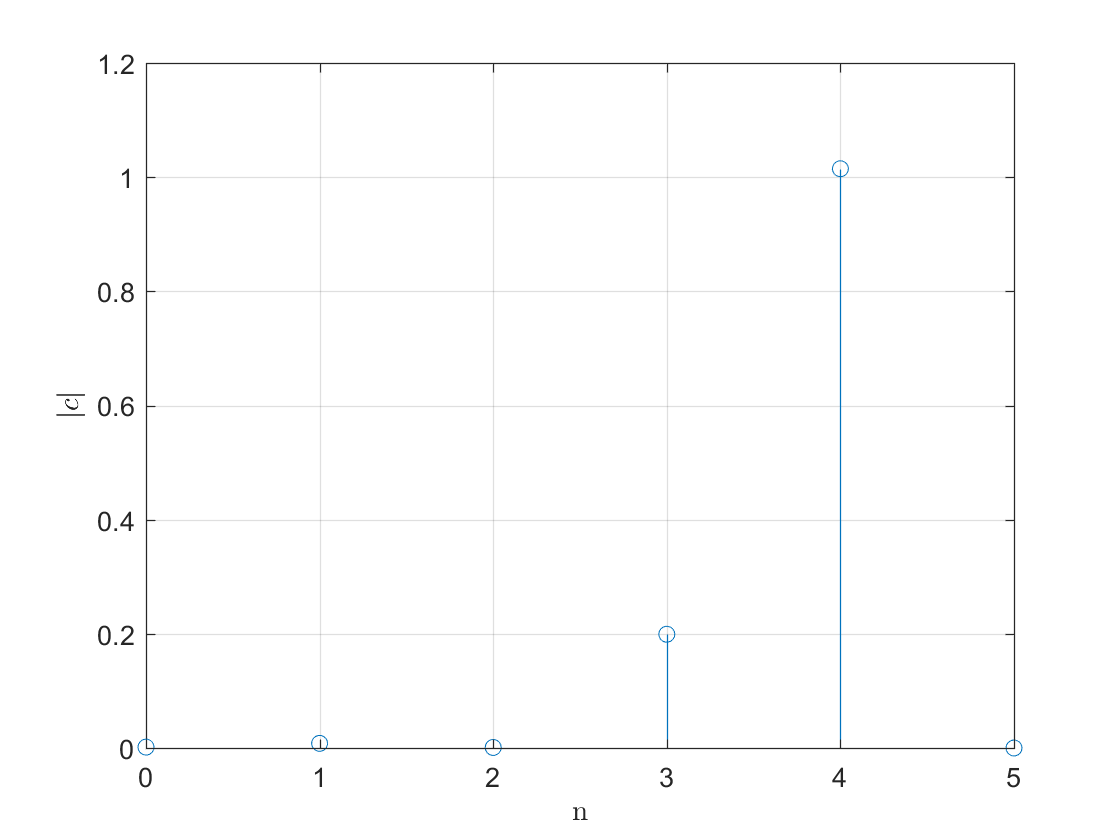
\includegraphics[width=8cm]{images/RecB_c}}
	\subfloat[Overall impulse response $\psi_i$.]{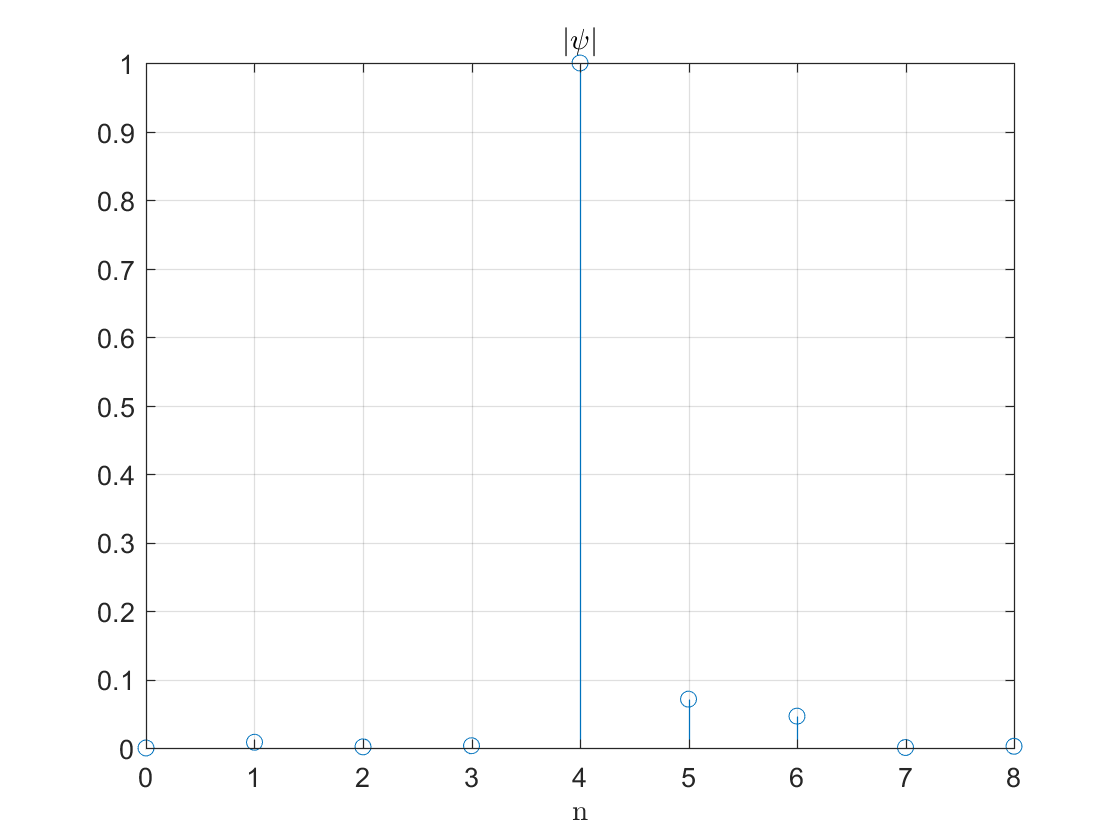
\includegraphics[width=8cm]{images/RecB_psi}}\quad
	\subfloat[Feedback filter $b$.]{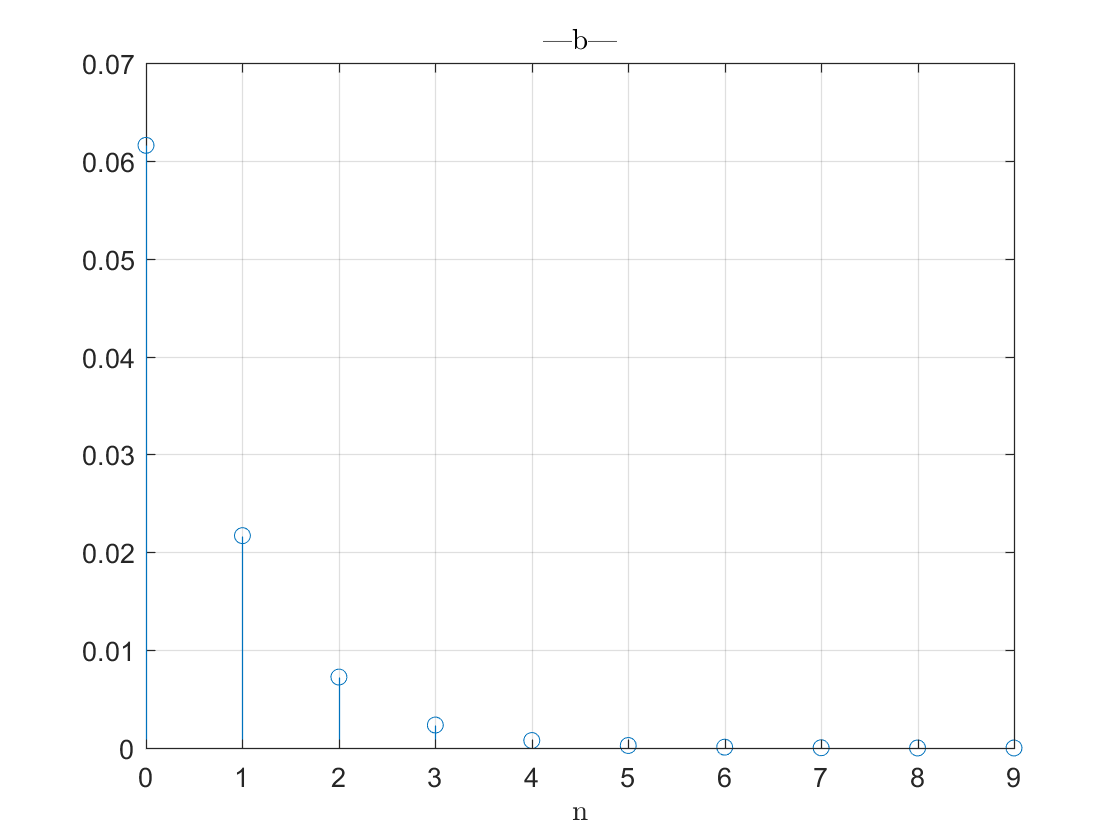
\includegraphics[width=8cm]{images/RecB_b}}
	\subfloat[Matched filter $g_m$.]{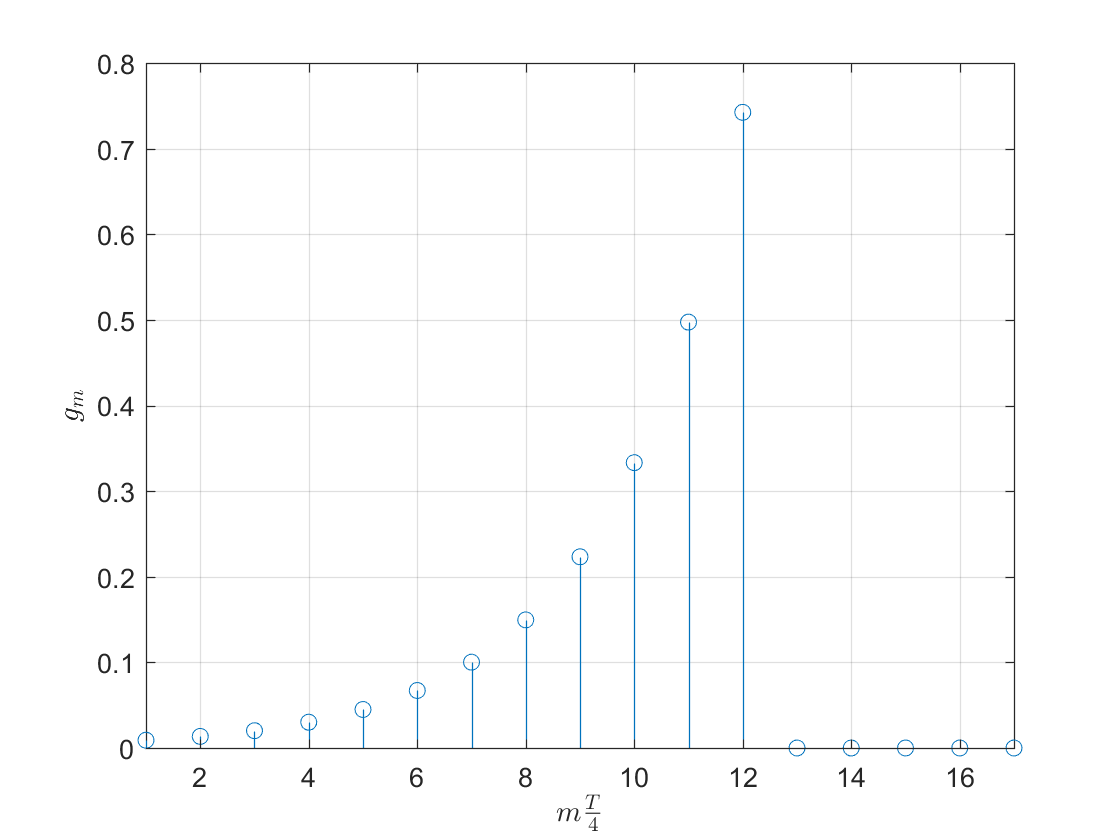
\includegraphics[width=8cm]{images/RecB_gm}}
	\caption{Coefficients for the DFE, overall impulse response and matched filter. Note that $g_m$ is the same as for receiver (a).}\label{filters_b}
\end{figure}



\clearpage
\subsection*{Receiver c}

\begin{figure}[H]
	\centering
	\begin{tikzpicture}[auto,>=latex']
	\tikzstyle{block} = [draw, rectangle, minimum height=1cm, minimum width=1cm]
	
	\node [coordinate, label={[label distance=0.2cm]180:$r_c(n \frac{T}{4})$}] (start) {};
	\node [block, right = 1cm of start] (gaa){$g_{AA}$};
	\node [coordinate, right = 0.75 cm of gaa] (c0) {};
	\node [coordinate, above = 0.5 cm of c0, label={[label distance=0.1cm]45:$t_0 + m \frac{T}{2}$} ] (c1) {};
	
	\node [coordinate, right = 1.2cm of gaa] (c2) {};
	
	\node [block, right = 1cm of c2] (gm){$g_M$};
	
	\node [block, right = 1cm of gm] (cfilter){$c$};
	
	\node [draw, circle,minimum size=0.5cm,inner sep=0pt, right = 1cm of cfilter] (sum){$+$};
	
	\node [coordinate, below = 1cm of sum] (c3) {};	
	
	\node [block, right = 2.5cm of sum] (detector){$\amalg$};
	
	\node [coordinate, right = 0.5cm of detector] (cfin) {};
	
	\node [coordinate, below = 1.254cm of cfin] (c6) {};
	
	\node [block, right = 1cm of c3] (b){$b$};	
	
	\node [coordinate, right = 1cm of detector, label={[label distance=0.1cm]0:$\hat{a}_{k-D}$}] (end){};
	
	\draw [->] (start) --node[label={[label distance=0.2cm]270:$\frac{T}{4}$}]{} (gaa);
	\draw [-] (gaa) --node[label={[label distance=0.2cm]270:$\frac{T}{4}$}]{} (c0);
	\draw [-] (c1) --node[]{} (c2);
	\draw [->] (c2) --node[label={[label distance=0.2cm]270:$\frac{T}{2}$}]{} (gm);
	\draw [->] (gm) --node[label={[label distance=0.2cm]270:$\frac{T}{2}$}]{} (cfilter);
	\draw [->] (cfilter) --node[label={[label distance=0.2cm]270:$T$}]{} (sum);
	\draw [->] (c3) --node[]{} (sum);
	\draw [-] (b) --node[]{} (c3);
	\draw [-] (c6) --node[]{} (b);
	\draw [-] (cfin) --node[label={[label distance=0.1cm]0:$T$}]{} (c6);
	\draw [->] (sum) --node[]{} (detector);
	\draw [->] (detector) --node[]{} (end);
	\end{tikzpicture}
	\caption{Model for the receiver (c).}
	\label{Receiver_c} 
\end{figure}

In this case the analog filter is replaced by a digital \textit{anti-aliasing} filter $g_{AA}$. The signal at the output is downsampled by a factor 2, then a cascade of a matched filter and a DFE  filter processes the signal and produces the output symbols $\hat{a}_{k-D}$. The filter $g_m$ is needed in order to allow the equalizer filter defined in Equation (\ref{c}) to act as a matched filter.\\
Note also that the filter $c$ is now works at T/2, so the new formulas to compute $\mathbf{c}_{opt}$ are now:

\begin{equation}
\mathbf{[R]}_{p,q} = \sigma_a^2 \left( \sum_{n=-\infty}^{+\infty}h_{2n-q}h^*_{2n-p}-\sum_{j=1}^{M_2}h_{j+D-q}h^*_{2(j+D)-p} \right) + r_{\tilde{w}}(p-q)
\end{equation}
\begin{equation}
\mathbf{[p]}_p = \sigma_a^2 h^*_{2D-p}, \quad\quad\quad\quad\quad\quad\quad\quad\quad\quad\quad p,q = 0,1,\dots,M_1-1
\end{equation}
In the following Table [\ref{gaa}] are reported the parameters for the anti-aliasing filter.\\
Since input signal frequency is periodic, the anti-aliasing filter will delete useful information, hence we expect worse performances than previous receivers.

\begin{table}[H]
	\centering
	\begin{tabular}{c | c}
		\toprule
		Parameter & Value \\
		\midrule
		Passband frequency $F_{p}$ & 0.45\\
		Stopband frequency $F_{s}$ & 0.55\\
		Passband ripple $\delta_{p}$ & 0.05\\
		Stopband ripple $\delta_{s}$ & 0.01\\
		\bottomrule			
	\end{tabular}
	\caption{Parameters of the anti-aliasing filter.}
	\label{gaa}
\end{table}
Frequency response of the anti-aliasing and of the matched filter are given in Figure [\ref{filters_c}].
\begin{figure}[H]
	\centering
	\subfloat[Frequency response of anti-aliasing filter.]{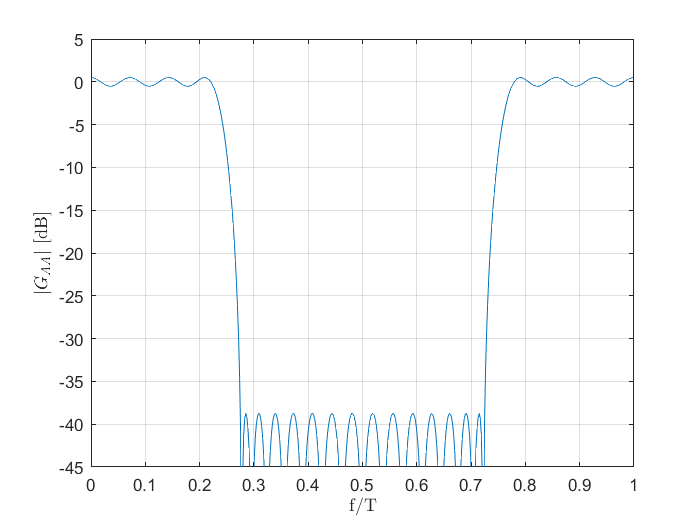
\includegraphics[width=8cm]{images/RecC_GAA}}
	\subfloat[Frequency response of matched filter.]{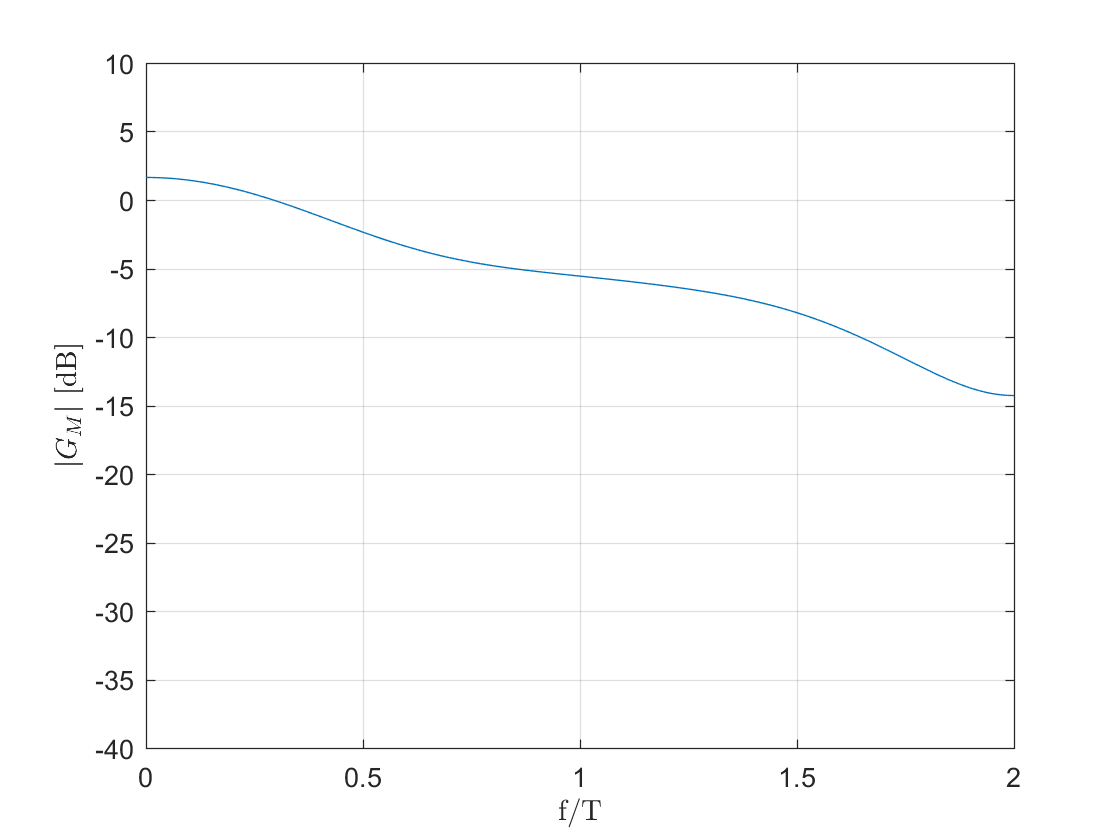
\includegraphics[width=8cm]{images/RecC_GM}}
	\caption{Anti-aliasing and matched filters of the Receiver (c).}\label{filters_c}
\end{figure}

Parameters $M_1$, $M_2$ and $D$ are chosen evaluating $J_{min}$. For values greater than $M_1=10$ and $D=4$ there is no noticeable improvement, so we decided to use these parameters.

\begin{figure}[H]
	\centering
	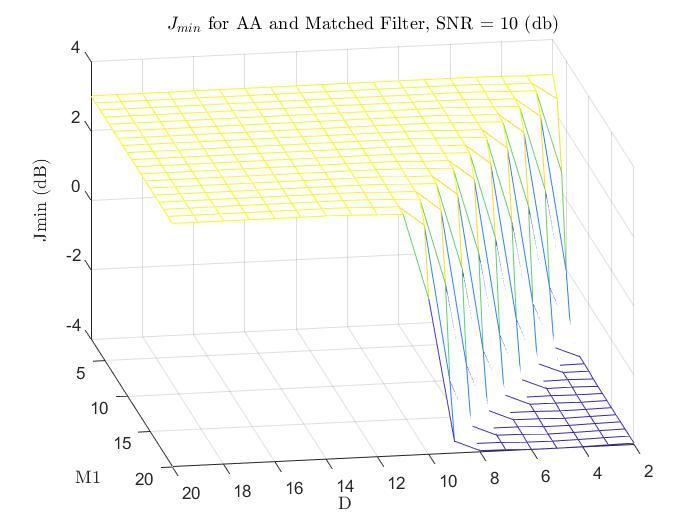
\includegraphics[width=7cm]{images/optimal_params_AntiAliasing}
	\caption{$J_{min}$ as a function of $M_1$ and $D$.}\label{j_min_aa}
\end{figure}

\begin{table}[H]
	\centering
	\begin{tabular}{c c c c}
		\toprule
		$\mathbf{\bar{t}_0}$ & $\mathbf{M_1}$ & $\mathbf{M_2}$ & \textbf{D}     \\
		\midrule
		21 & 10 & 24 & 4 \\
		\bottomrule			
	\end{tabular}
	\caption{Parameters of the Receiver (c).}
	\label{Tab_c}
\end{table}

In Figure [\ref{rec_c}] are reported the coefficients for the DFE and the overall impulse response.
\begin{figure}[H]
	\centering
	\subfloat[Feedforward filter $c$.]{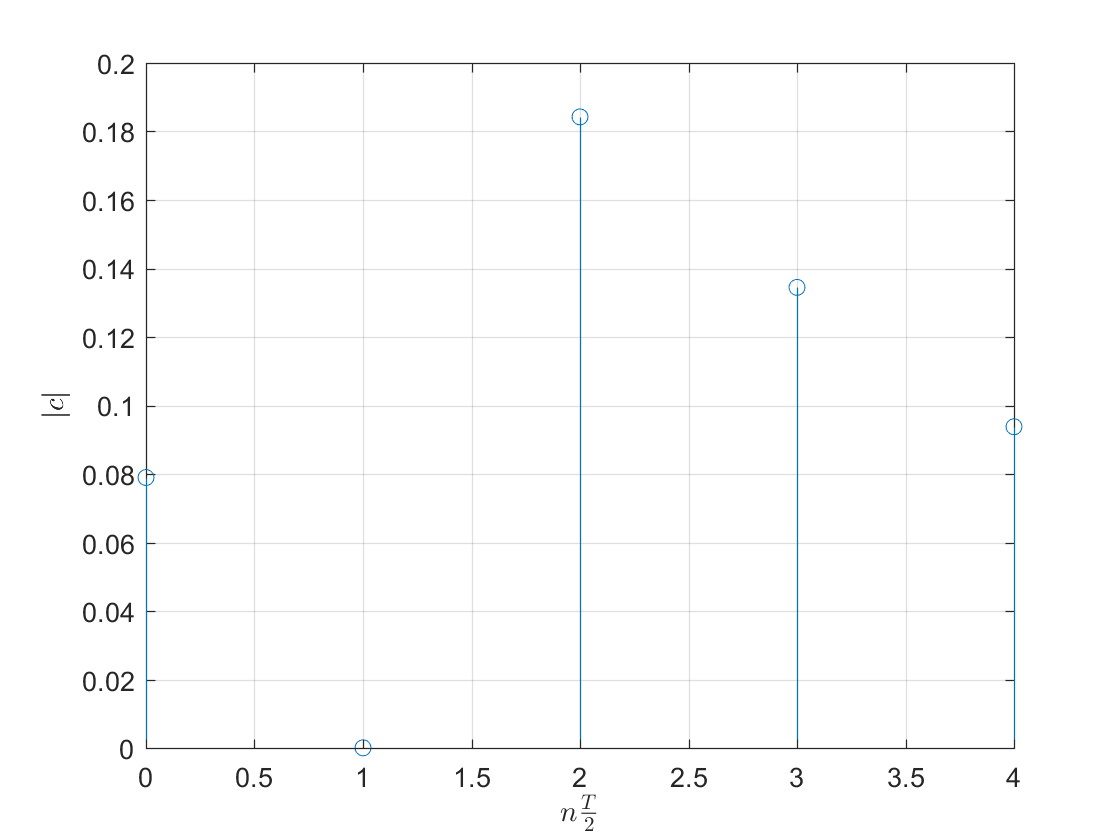
\includegraphics[width=7cm]{images/RecC_c}}
	\subfloat[Overall impulse response $\psi_i$.]{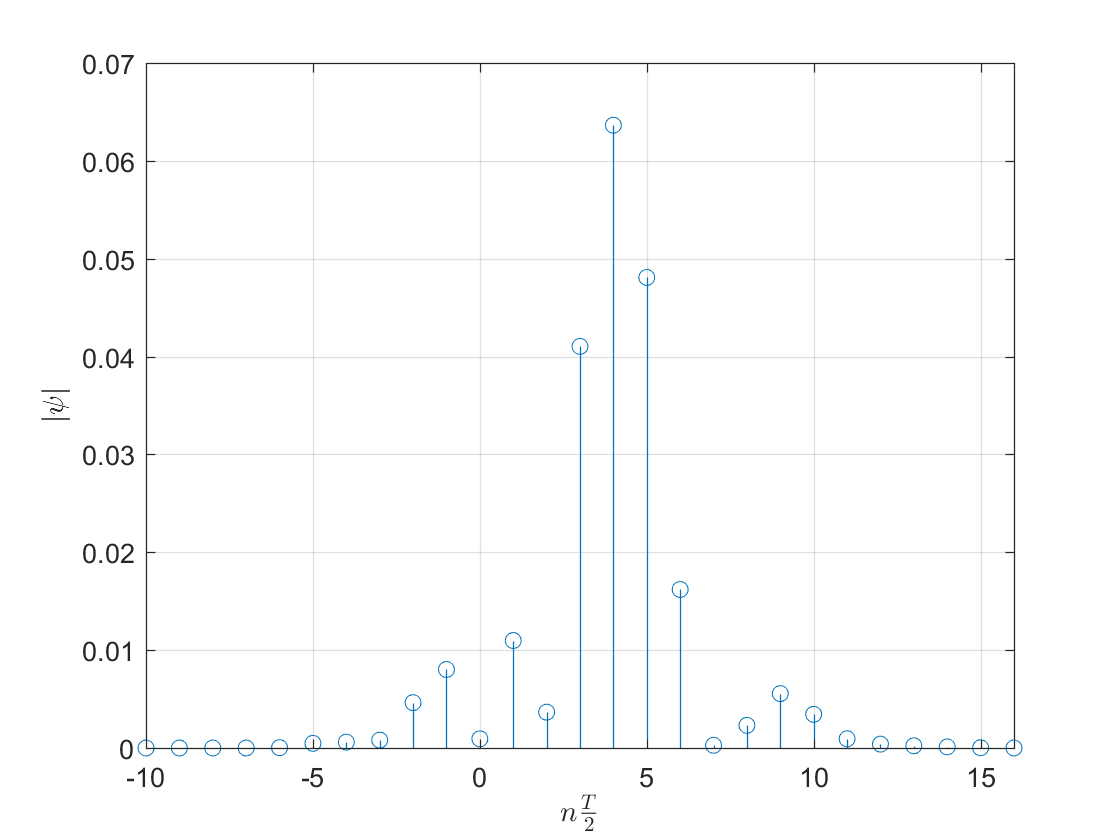
\includegraphics[width=7cm]{images/RecC_psi}}\quad
	\subfloat[Feedback filter $b$.]{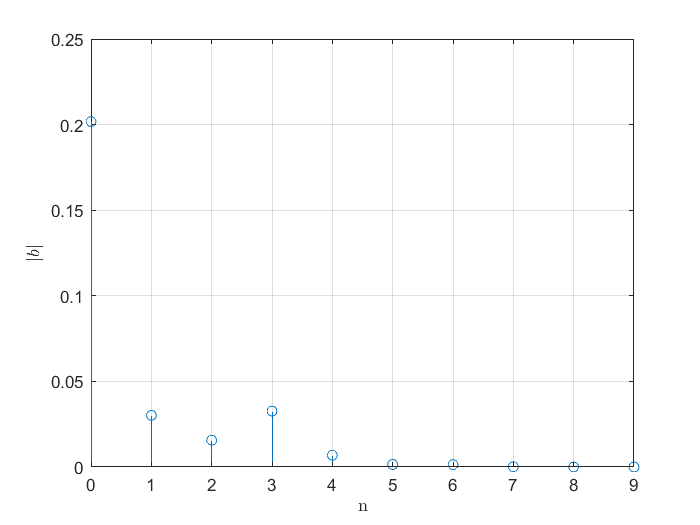
\includegraphics[width=7cm]{images/RecC_b}}
	\caption{Coefficients of the FF filter $c$, of the overall impulse response $\psi_i$ and of the FB filter $b$.}\label{rec_c}
\end{figure}

\clearpage
\subsection*{Receiver d}

\begin{figure}[H]
	\centering
	\begin{tikzpicture}[auto,>=latex']
	\tikzstyle{block} = [draw, rectangle, minimum height=1cm, minimum width=1cm]
	
	\node [coordinate, label={[label distance=0.2cm]180:$r_c(n \frac{T}{4})$}] (start) {};
	\node [block, right = 1cm of start] (gaa){$g_{AA}$};
	\node [coordinate, right = 0.75 cm of gaa] (c0) {};
	\node [coordinate, above = 0.5 cm of c0, label={[label distance=0.1cm]45:$t_0 + m \frac{T}{2}$} ] (c1) {};
	
	\node [coordinate, right = 1.2cm of gaa] (c2) {};
	
	\node [block, right = 1cm of c2] (cfilter){$c$};
	
	\node [draw, circle,minimum size=0.5cm,inner sep=0pt, right = 1cm of cfilter] (sum){$+$};
	
	\node [coordinate, below = 1cm of sum] (c3) {};	
	
	\node [block, right = 2.5cm of sum] (detector){$\amalg$};
	
	\node [coordinate, right = 0.5cm of detector] (cfin) {};
	
	\node [coordinate, below = 1.254cm of cfin] (c6) {};
	
	\node [block, right = 1cm of c3] (b){$b$};	
	
	\node [coordinate, right = 1cm of detector, label={[label distance=0.1cm]0:$\hat{a}_{k-D}$}] (end){};
	
	\draw [->] (start) --node[label={[label distance=0.2cm]270:$\frac{T}{4}$}]{} (gaa);
	\draw [-] (gaa) --node[label={[label distance=0.2cm]270:$\frac{T}{4}$}]{} (c0);
	\draw [-] (c1) --node[]{} (c2);
	\draw [->] (c2) --node[label={[label distance=0.2cm]270:$\frac{T}{2}$}]{} (cfilter);
	\draw [->] (cfilter) --node[label={[label distance=0.2cm]270:$T$}]{} (sum);
	\draw [->] (c3) --node[]{} (sum);
	\draw [-] (b) --node[]{} (c3);
	\draw [-] (c6) --node[]{} (b);
	\draw [-] (cfin) --node[label={[label distance=0.1cm]0:$T$}]{} (c6);
	\draw [->] (sum) --node[]{} (detector);
	\draw [->] (detector) --node[]{} (end);
	\end{tikzpicture}
	\caption{Model for the receiver (d).}
	\label{Receiver_d} 
\end{figure}

The same configuration of receiver (c) is here simulated without the match filter at the input of the DFE. In this case we expect lower performances with respect to the previous configuration, since the equalizing filter is not matched with the impulse response at its input.\\
For this receiver we used the same parameters the previous one, since the cost function has similar behavior.

\begin{figure}[H]
	\centering
	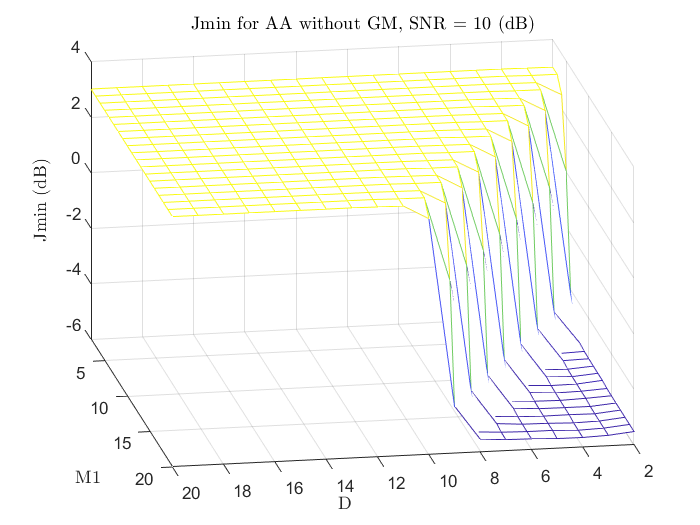
\includegraphics[width=8cm]{images/optimal_params_AntiAliasingNoMF}
	\caption{$J_{min}$ as a function of $M_1$ and $D$.}\label{j_min_aa_nomf}
\end{figure}

\begin{table}[H]
	\centering
	\begin{tabular}{c c c c}
		\toprule
		$\mathbf{\bar{t}_0}$ & $\mathbf{M_1}$ & $\mathbf{M_2}$ & \textbf{D}     \\
		\midrule
		21 & 10 & 17 & 4 \\
		\bottomrule			
	\end{tabular}
	\caption{Parameters of the Receiver (d).}
	\label{Tab_d}
\end{table}

The following filters were computed.

\begin{figure}[H]
	\centering
	\subfloat[Feedforward filter $c$.]{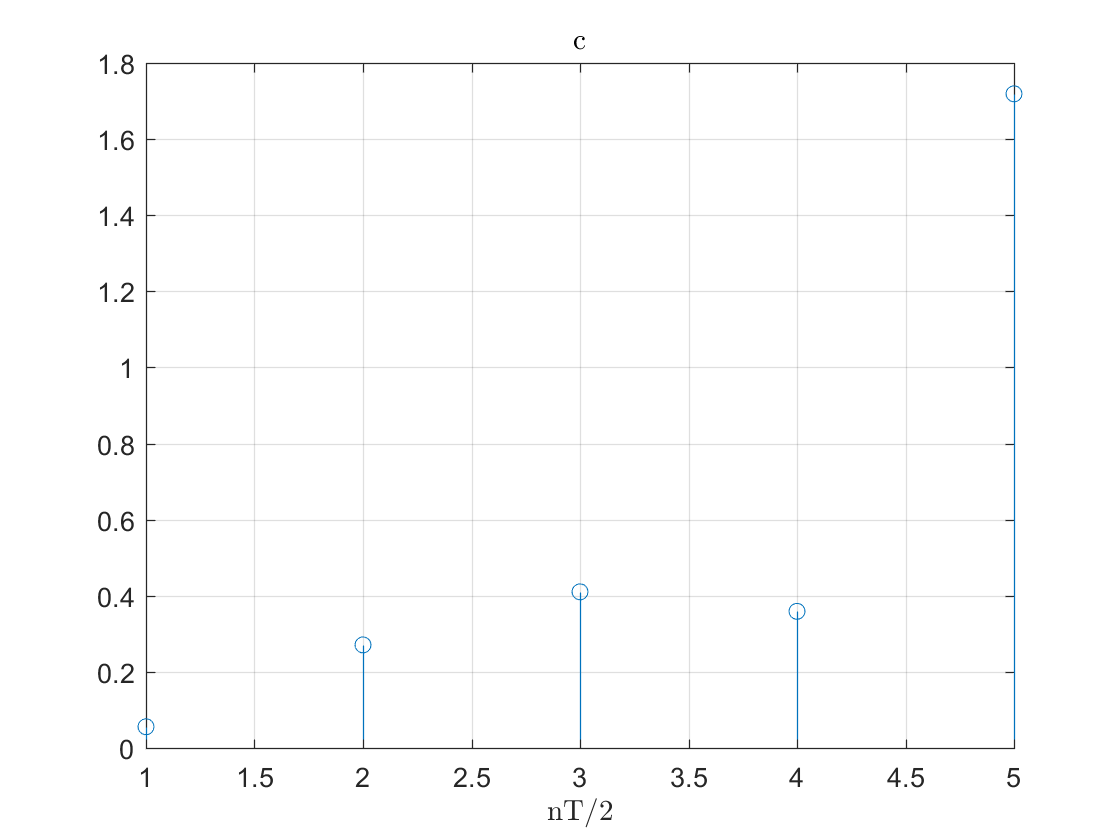
\includegraphics[width=8cm]{images/RecD_c}}
	\subfloat[Overall impulse response $\psi_i$.]{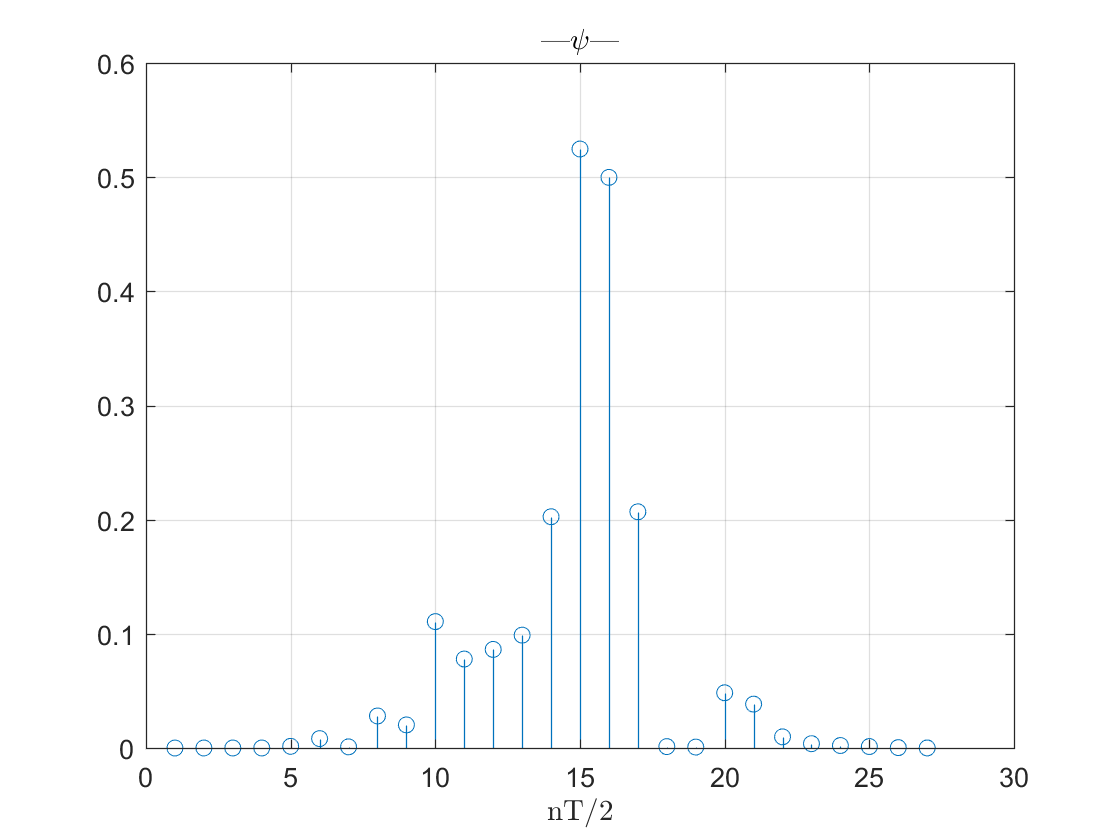
\includegraphics[width=8cm]{images/RecD_psi}}\quad
	\subfloat[Feedback filter $b$.]{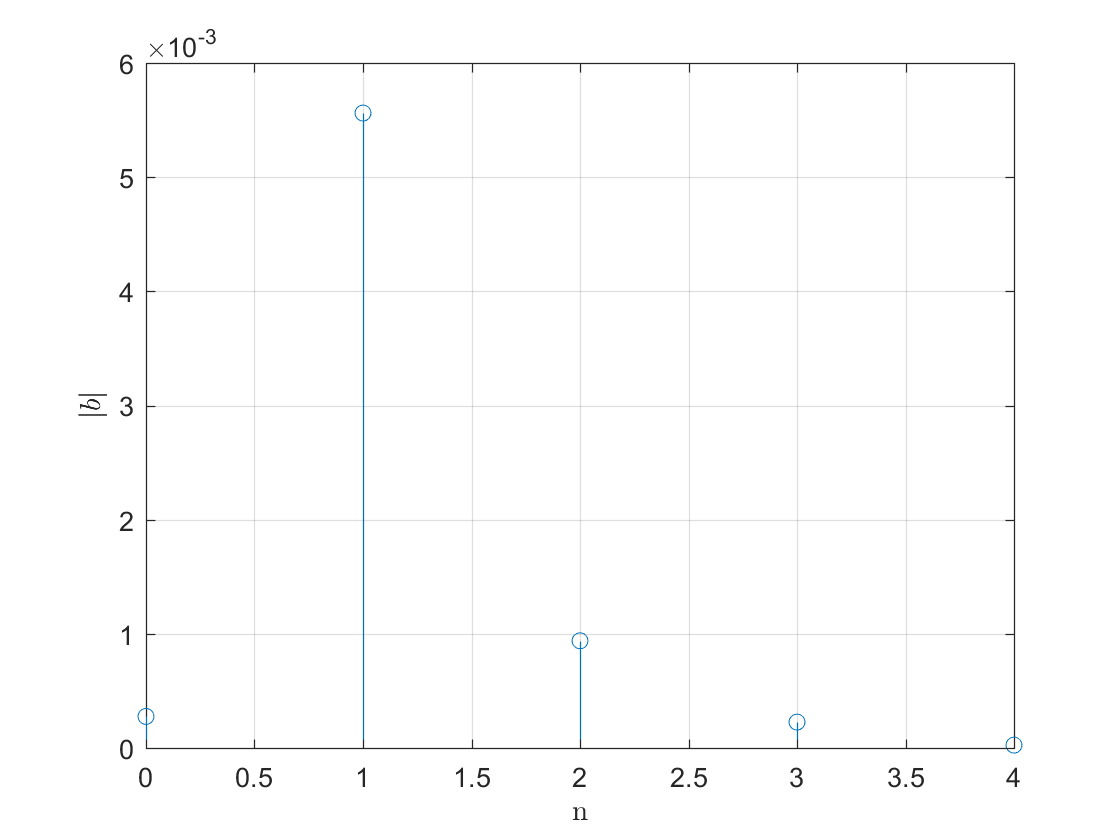
\includegraphics[width=9cm]{images/RecD_b}}
	\caption{Coefficients of the FF filter $c$, of the overall impulse response $\psi_i$ and of the FB filter $b$.}\label{rec_d}
\end{figure}



\clearpage
\subsection*{Receiver e}

\begin{figure}[H]
	\centering
	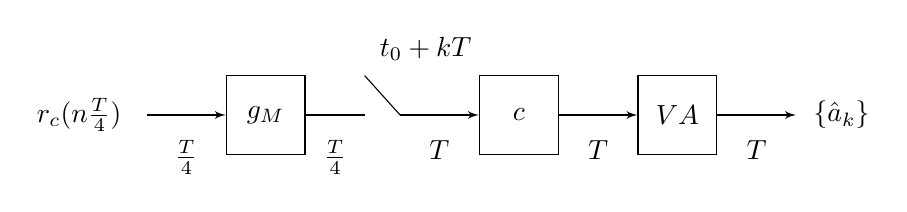
\begin{tikzpicture}[auto,>=latex']
	\tikzstyle{block} = [draw, rectangle, minimum height=1cm, minimum width=1cm]
	
	\node [coordinate, label={[label distance=0.2cm]180:$r_c(n \frac{T}{4})$}] (start) {};
	\node [block, right = 1cm of start] (matchedf){$g_M$};
	\node [coordinate, right = 0.75 cm of matchedf] (c0) {};
	\node [coordinate, above = 0.5 cm of c0, label={[label distance=0.1cm]45:$t_0 + kT$} ] (c1) {};
	
	\node [coordinate, right = 1.2cm of matchedf] (c2) {};
	
	\node [block, right = 1cm of c2] (cfilter){$c$};
	\node [block, right = 1cm of cfilter] (viterbi){$VA$};
	
	\node [coordinate, right = 1cm of viterbi, label={[label distance=0.1cm]0:$\{\hat{a}_k\}$}] (end){};
	
	\draw [->] (start) --node[label={[label distance=0.2cm]270:$\frac{T}{4}$}]{} (matchedf);
	\draw [-] (matchedf) --node[label={[label distance=0.2cm]270:$\frac{T}{4}$}]{} (c0);
	\draw [-] (c1) --node[]{} (c2);
	\draw [->] (c2) --node[label={[label distance=0.2cm]270:$T$}]{} (cfilter);
	\draw [->] (cfilter) --node[label={[label distance=0.2cm]270:$T$}]{} (viterbi);
	\draw [->] (viterbi) --node[label={[label distance=0.2cm]270:$T$}]{} (end);
	
	\end{tikzpicture}
	\caption{Model for the receiver (e).}
	\label{Receiver_e} 
\end{figure}

Here the receiver uses the channel as given by $\psi_D$,$\psi_{D+1}$,\dots,$\psi_{D+M_2}$ of Receiver (b) and performs the maximum likelihood detection through the Viterbi algorithm. \\
The state of the \textit{finite state machine} associated with the algorithm at time $k=0,\dots,K-1$ is 

\begin{equation}
\textbf{s}_k = a_{k+L_1},a_{k+L_1-1},\dots,a_{k},\dots,a_{k-L_2+1} 
\end{equation}

where $K$ is the length of the input sequence, so the total number of states is $N_s = M^{L_1+L_2}$.\\
The set of the states $\mathcal{S}$ is the set of the possible values of $\textbf{s}_k$, such that $\mathbf{s}_k \in \{ \mathbf{\sigma}_1,\mathbf{\sigma}_2,\dots,\mathbf{\sigma}_{N_s} \}$. With each state $\mathbf{\sigma}_j$, at instant $k$ the algorithm computes the following quantities:

\begin{enumerate}
	\item The path metric, $\Gamma(\mathbf{s}_k=\mathbf{\sigma}_j)$;
	\item The survivor sequence, $\mathcal{L}(\mathbf{s}_k=\mathbf{\sigma}_j)$.
\end{enumerate}

These quantities are computed recursively. Starting from $k=0$, the procedure is repeated until $k=K-1$. The optimum sequence of states is given by the survivor sequence $\mathcal{L}(\mathbf{s}_{K-1}=\mathbf{\sigma}_{j,opt})$ associated with $\mathbf{s}_{K-1}=\mathbf{\sigma}_{j,opt}$ having minimum cost.

\clearpage
\subsection*{Receiver f}

\begin{figure}[H]
	\centering
	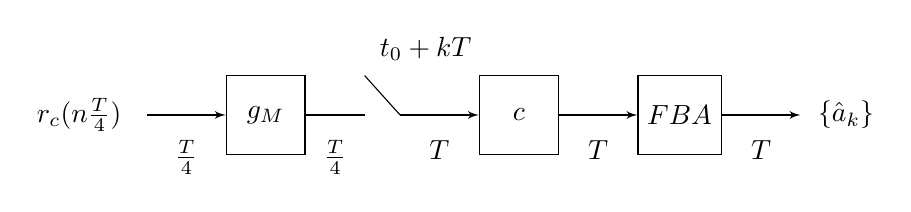
\begin{tikzpicture}[auto,>=latex']
	\tikzstyle{block} = [draw, rectangle, minimum height=1cm, minimum width=1cm]
	
	\node [coordinate, label={[label distance=0.2cm]180:$r_c(n \frac{T}{4})$}] (start) {};
	\node [block, right = 1cm of start] (matchedf){$g_M$};
	\node [coordinate, right = 0.75 cm of matchedf] (c0) {};
	\node [coordinate, above = 0.5 cm of c0, label={[label distance=0.1cm]45:$t_0 + kT$} ] (c1) {};
	
	\node [coordinate, right = 1.2cm of matchedf] (c2) {};
	
	\node [block, right = 1cm of c2] (cfilter){$c$};
	\node [block, right = 1cm of cfilter] (fba){$FBA$};
	
	\node [coordinate, right = 1cm of fba, label={[label distance=0.1cm]0:$\{\hat{a}_k\}$}] (end){};
	
	\draw [->] (start) --node[label={[label distance=0.2cm]270:$\frac{T}{4}$}]{} (matchedf);
	\draw [-] (matchedf) --node[label={[label distance=0.2cm]270:$\frac{T}{4}$}]{} (c0);
	\draw [-] (c1) --node[]{} (c2);
	\draw [->] (c2) --node[label={[label distance=0.2cm]270:$T$}]{} (cfilter);
	\draw [->] (cfilter) --node[label={[label distance=0.2cm]270:$T$}]{} (fba);
	\draw [->] (fba) --node[label={[label distance=0.2cm]270:$T$}]{} (end);
	
	\end{tikzpicture}
	\caption{Model for the receiver (f).}
	\label{Receiver_f} 
\end{figure}
Still using the channel as given in the previous section, the signal at the output of the $c$ filter is now processed by a \textit{Forward-Backward algorithm} exploiting the Max-Log-MAP to detect the received symbols $\hat{a}_k$. For each instant $k=0,1,\dots,K-1$, the algorithm performs the computation of five metrics, respectively:

\begin{enumerate}
	\item The channel transition metric, $c_k(i,j)$, $i,j=1,\dots,N_s$;
	\item The Backward metric, $\tilde{b}_k(i)$, $i=1,\dots,N_s$;
	\item The Forward metric, $\tilde{f}_k(j)$, $j=1,\dots,N_s$;
	\item The State metric, $\tilde{v}_k(i)$, $i=1,\dots,N_s$;
	\item The Log-Likelihood function of the isolated symbol $\tilde{l}_k(\beta)= \max\limits_{\overset{i\in[1,\dots,N_s],} {[\sigma_i]_1=\beta}}=\tilde{v}_k(i)$.
\end{enumerate}

The actual state metric in linear domain is defined as $V_k(i) = P[\mathbf{s}_k=\mathbf{\sigma}_i|\mathbf{z}^{K-1}_0=\mathbf{\rho}^{K-1}_0]$ and expresses the probability of being in state $\mathbf{\sigma}_i$ at instant $k$, given the whole observation $\mathbf{\rho}^{K-1}_0$. In the LOG-MAP criterion, the logarithmic variables are indicated with the corresponding lower-case vector, such that $v_k(i)=\ln V_k(i)$. The \textit{log-likelihood} function is then computed as

\begin{equation}
l_k(\beta) = \ln L_k(\beta) = \ln\left(\sum_{\overset{i=1}{[\sigma_i]_1=\beta}}^{N_s}e^{v_k(i)}\right)\simeq \max\limits_{\overset{i\in[1,\dots,N_s],} {[\sigma_i]_1=\beta}}v_k(i)
\end{equation}

from which if follows the approximated likelihood function

\begin{equation}
\tilde{l}_k(\beta) = \max\limits_{\overset{i\in[1,\dots,N_s],} {[\sigma_i]_1=\beta}}v_k(i)
\end{equation}

The detected symbol is then evaluated using the MAX-LOG-MAP criterion:

\begin{equation}
\hat{a}_{k+L_1} = \argmax_{\beta \in \mathcal{A}} \tilde{l}_k(\beta)
\end{equation}

\clearpage
\section*{SER comparison}
For each of the different configurations previously described, the symbol error probability is evaluated by simulations with different values of the SNR $\Gamma$.\\
This is computed by counting the number of errors at the output of each receiver after the transmission of a PN sequence of length $L = 2^{20}-1$, where couples of generated bits are previously mapped into QPSK symbols. \\ 
The results given are obtained taking the average over 10 independent realizations of the noise.

\begin{figure}[H]
	\centering
	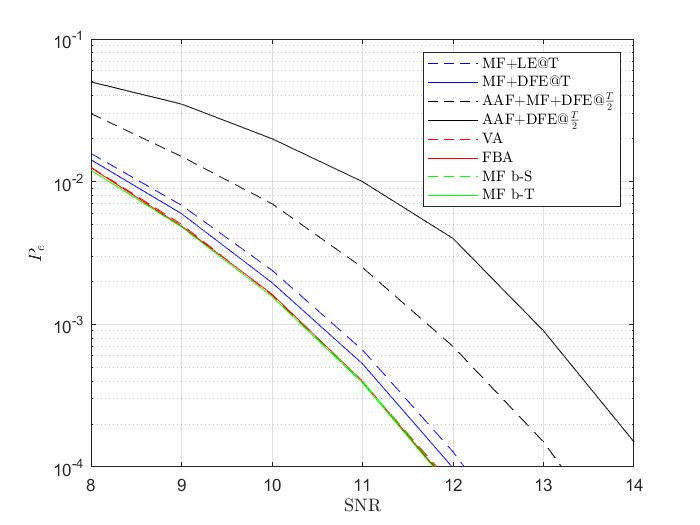
\includegraphics[width=15cm]{images/PevsGamma}
	\caption{Simulated BER for the different receivers at different SNR values.}\label{Pe}
\end{figure}

As expected, the Viterbi and the FBA algorithms yield to a $Pe$ which is very close to the bound. On the other hand, these performances are reached with a high computational cost. Even the LE and the DFE offers a reliable communication in term of error probability, which may be explained observing that the overall impulse response $\psi$ has a very good shape in terms of ISI cancellation: all the precursors are cancelled out by the $c$ filter. Finally, the receivers with the anti-aliasing filter shows worse performances due to the fact that the filter truncates the useful signal. These are slightly improved by using a $g_m$ at the input of the equalizing filter, forcing it to act also as a matched filter as in the case of Receiver c.

\end{document}